\section{The Resistor Color Code}
\label{resistor_code}

The table below shows how to use the resistor color code to determine the value of a resistor with colored bands.  In all cases, the digits come first, then the multiplier band, then a ``tolerance'' band. 


{\centering 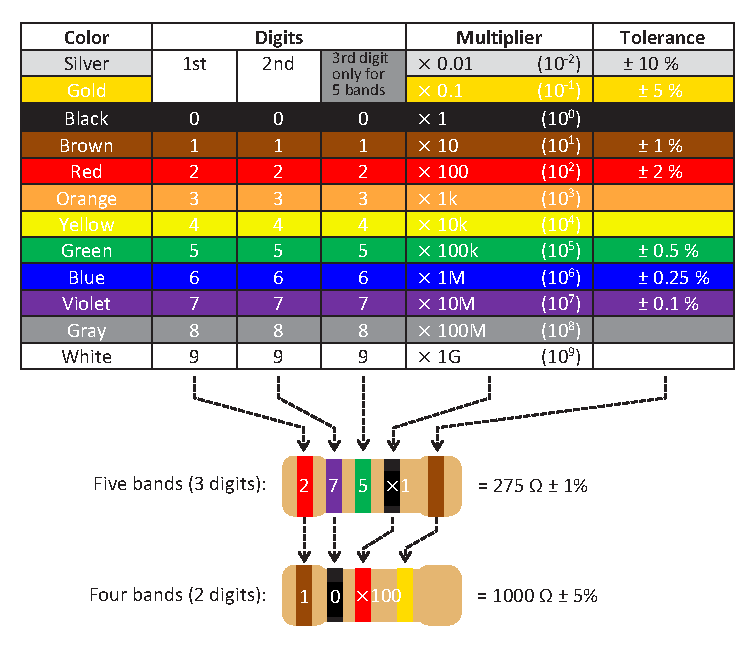
\includegraphics{appendices/resistor_code/resistor_table.eps} \par}
\index{color page}

The tolerance band tells you something like the ``uncertainty'' of the resistance, but the values are given very conservatively because the manufacturer \textit{guarantees} that the value will be within the stated tolerance.  The four-band resistor above is \textit{guaranteed} to be between $950~\Omega$ and $1050~\Omega$.  In practice, you will \textit{never} find a 5\% resistor that is actually off by that much.


\medskip
\textbf{Which Direction to Read? Several possible clues:}
\begin{itemize}[nosep]
\item Sometimes the first digit is closer to the end of the resistor than the tolerance band.  If so, start there.
\item Sometimes there is extra space between the multiplier and tolerance bands, as in the drawings above.  If you see that space, start on the other side.
\item Gold and Silver are never digits; they are always tolerance bands.  If you see gold or silver, start on the other side.
\end{itemize}

\medskip
\textbf{Variations and Warnings}

There are rare variations to this scheme.  Occasionally a final band will denote the temperature coefficient or a failure rate.  Also, be warned: on very small bands, it is easy to confuse orange/red, red/brown, or violet/gray.  Fortunately, you can always measure a resistor with your multimeter.  

\medskip
\textbf{Mnemonic Devices}

There are several fun phrases (and some not so fun ones) you can memorize to help you remember the order of the colors.   In the ones below, the vowels also help distinguish between Black/Brown/Blue and Green/Gray.
\begin{itemize}[nosep]
\item \textbf{Ba}d \textbf{Bo}sses \textbf{R}ely \textbf{O}n \textbf{Y}oung \textbf{Gee}ks, \textbf{Bu}t \textbf{V}alue \textbf{Grea}t \textbf{W}ork.
\item \textbf{Bla}nd \textbf{Bo}oks \textbf{R}eportedly \textbf{O}ptimize \textbf{Y}our \textbf{GRE}, \textbf{Bu}t \textbf{V}ideo \textbf{Ga}mes \textbf{W}on't.
\end{itemize}

